\section{DATASET DESCRIPTION AND PREPROCESSING PROCEDURES}
\label{DATASET DESCRIPTION AND PREPROCESSING PROCEDURES}
Although MFL data looks quite similar for different pipes and ILI tool types, it can differ significantly.
The data mainly depends on pipe size, wall width, sensors geometry, and other geometric characteristics.
Moreover, ILI tools differ a lot for different pipe sizes.
Therefore, the repeatability of the results for different datasets should be investigated additionally.
Following, we provide dataset characteristics, which are also presented in Table~\ref{tab:dataset}.
We have data collected from the 219 mm in diameter pipe.
MFL dataset provides information about a single inspection tool run.
Dataset has 64 features collected as an array with a constant step along with the ILI tool movement inside the pipe.
Dataset has 4470704 samples that represent 15162.85 meters long pipeline part.
Sample values vary from 0 to 4095 units.
It has 745 defects of different types and 1462 welds, 34 of which are defected.
Fig.~\ref{ris:defect_example} shows examples of healthy data, data with a weld, and with a defect.
Attached to the dataset technical report contains information about welds and defects location, defects types, sizes, and other related characteristics.
\begin{table}[!htb]
	\caption{Dataset characteristics.}
	\begin{center}
		\small
		\begin{tabular}{  c | c   }
			\hline
			Parameter & Value \\
			\hline
			Pipeline diameter, mm &  219 \\
			Pipeline length, m &  15162.85 \\
			Number of samples &  4470704 \\
			Number of features & 64 \\
			Min value & 0 \\
			Max value & 4095 \\
			Mean value &   \\
			Number of defects/welds & 745/1462 \\
			\hline
		\end{tabular}
		\label{tab:dataset}
	\end{center}
\end{table}

\begin{figure}[ht]
	\center{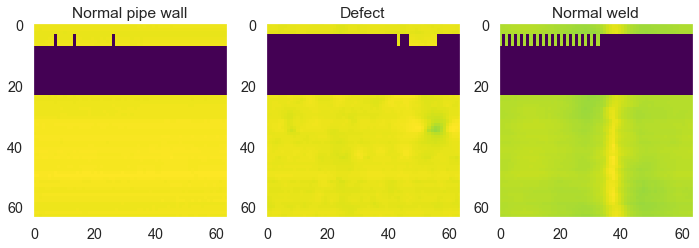
\includegraphics[scale=0.4]{pictures/1.png}}
	\caption{Example of the MFL data}
	\label{ris:defect_example}
\end{figure}

Raw data has several issues that don't allow us to solve CV problems without proper preprocessing.
They are:
\begin{enumerate}
	\item Sensors malfunctions (zeroed values cause bold horizontal line in Fig.~\ref{ris:defect_example});
	\item Displaced origins between data and reports coordinates;
	\item Inaccurate annotations, e.g., missed defects, wrong defect location, etc.
	\item No annotated data for the segmentation task.
\end{enumerate}

\subsubsection{Sensors malfunctions problem}
To deal with sensors malfunctions we suppose to fill the gaps (zeroed values) with values calculated by different methods.
Additionaly, we will consider values less than 2000 abnormal and replace them with zeroes during the preprocessing.
\begin{enumerate}
	\item Abnormal values are equal to 0. Then Min-Max scaling to $[0.5:1]$ range.
	\item Abnormal values are equal to the mean of normal values from one picture. Then Min-Max scaling.
	\item Abnormal values are equal to the mean of normal values over the column. Then Min-Max scaling.
	\item Abnormal values are equal to the mean of neighboring sensors over the column. Then Min-Max scaling.
	\item Abnormal values are equal to the interpolation results over the column. Then Min-Max scaling.
	\item Rerange initial set of values to 0...255 uint8 range.
	\item Rerange initial set of values to 0...1 float range \\ 
	(Fig.~\ref{ris:preproc_fun}). Such a specific function due to the range of normal operation of the sensor from 2500 to 3500 units.
\end{enumerate}

\begin{figure}[ht]
	\center{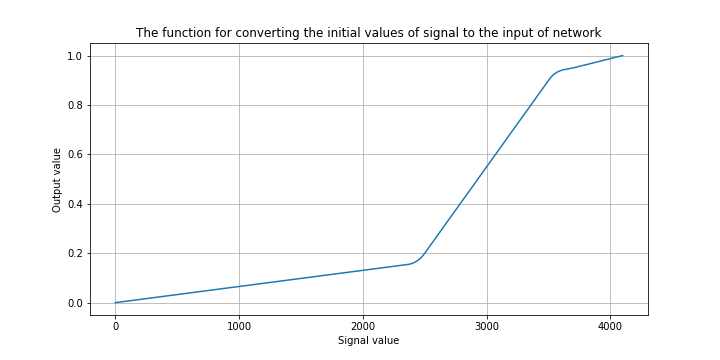
\includegraphics[scale=0.42]{pictures/preproc_fun.png}}
	\caption{The function for converting the initial values of signal to the input of network}
	\label{ris:preproc_fun}
\end{figure}

The results of all applied methods are presented in Fig.~\ref{ris:filling_example}.
\begin{figure}[ht]
	\center{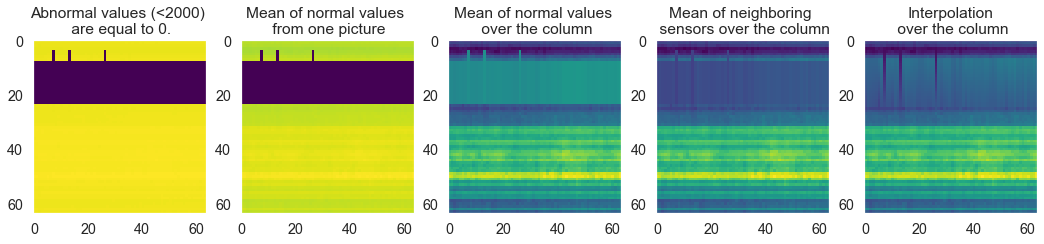
\includegraphics[scale=0.37]{pictures/2.png}}
	\caption{Comparison of methods for missing values filling}
	\label{ris:filling_example}
\end{figure}

Min-Max scaling can be applied using whole dataset or just one image.
Both approaches will be compared during the experiment conducting.

Since the ILI tool location data did not match the defect location data from the report, it was necessary to merge the data. The key factor here turned out to be that signal values from magnetic flux sensors grow at the weld site (Figure \ref{ris:prepr}). 

\begin{figure}[!h]
	\center{\includegraphics[width=0.82\linewidth]{pictures/prepr.png}}
	\caption{Location of a weld. The black vertical line is a weld, according to the report. Other lines are values from sensors.}
	\label{ris:prepr}
\end{figure}
The solution was to find the locations of the maxima of sensors data values and then to combine it with the weld coordinates.

\subsubsection{Manual annotations for the segmentation task}
Since there was no annotated data for the segmentation problem, it was necessary to annotate it manually (Figure \ref{ris:annot}). The characteristics of the obtained dataset can be seen in Table~\ref{tab:alg1}.

\begin{figure}[ht]
	\center{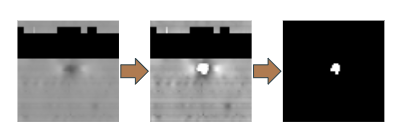
\includegraphics[scale=0.70]{pictures/annot.png}}
	\caption{The methodology for obtaining the mask}
	\label{ris:annot}
\end{figure}

\subsubsection{Inaccurate annotations problem}
This problem is a common one for oil and gas pipeline nondestructive testing \cite{Khodayari-Rostamabad2009}.
It appears to be a lot of missing defects that affect the quality of the problem.
Besides, there are wrong defect types and locations.
To eliminate wrong location issue, we additionaly searched extremums around the provided location and chose the defects or welds taking into account new coordinates.

\subsubsection{Augmentation}
Although we have a lot of data, we don't have a lot of defects and welds in comparison with healthy pipe wall instances.
We use the augmentation procedure to balance classes of pictures and increase the model's quality by increasing the number of pictures in small classes (defects, welds).
As an augmentation tool we use Albumentations library \cite{buslaev2020albumentations}.
All applied augmentations both for welds and defects are presented in Table~\ref{tab:aug}.
Applied augmentations details are presented in \cite{buslaev2020albumentations} and references therein.

\begin{table}[!htb]
	\caption{Applied augmentations.}
	\begin{center}
		\small
		\begin{tabular}{ c | c | c  }
			\hline
			Augmentation Types & Pipelines (welds) & Pipelines (defects) \\
			\hline
			Rotate90 &  - & \checkmark \\
			Rotate180 & \checkmark & \checkmark \\
			Rotate270 &  - & \checkmark \\
			VerticalFlip & \checkmark & \checkmark \\
			HorizontalFlip & \checkmark & \checkmark \\
			ElasticTransform & \checkmark & \checkmark \\
			GridDistortion & \checkmark & \checkmark \\
			OpticalDistortion & \checkmark & \checkmark \\
			Transpose & - & \checkmark \\
			RandomRotate90 &  - & \checkmark \\
			\hline
		\end{tabular}
		\label{tab:aug}
	\end{center}
\end{table}

Examples of augmentations are shown in Fig.~\ref{ris:aug_example}.
\begin{figure}[ht]
	\center{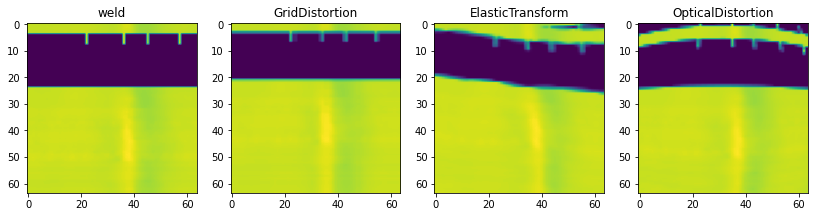
\includegraphics[scale=0.45]{pictures/4.png}}
	\caption{Examples of the augmented weld image}
	\label{ris:aug_example}
\end{figure}


The characteristics of the pipeline defects dataset are described in Table \ref{tab:alg1}, where * symbol indicates a random call function 5 and 6 from the defects augmentation list, so the exact number is unknown.
\begin{table}[!htb]
	\caption{\label{tab:alg1}Dataset size for pipeline defects detection and segmentation problems}
	\begin{center}
		\small
		\begin{tabular}{ c | c  c  c | c  c }
			\multicolumn{1}{c}{} & \multicolumn{3}{c}{Classification} & \multicolumn{2}{c}{Segmentation} \\
			\hline
			Data & Healthy & Defect & Weld & Healthy & Defect \\
			\hline
			\multicolumn{6}{c}{Before augmentation}  \\
			\hline
			Train  & 11106 & 569 & 1130 & 181 & 450 \\
			Validation & 584 & 142 & 282 & 33 & 111 \\
			\hline
			\multicolumn{6}{c}{After augmentation}  \\
			\hline
			Train  & 11106 & 8535 & 11300 & * & * \\
			Validation & 584 & 142 & 282 & * & * \\
			\hline
		\end{tabular}
	\end{center}
\end{table}

\section{METHODS}
\label{METHODS}
Pipeline defect detection is composed of two problems. First, the defect should be detected, and further, it should be evaluated using segmentation results.
We propose here a novel CNN architecture for image classification.
Additionally, we present the existing architectures that achieve best results in the MFL and X-ray data classification problems.

\subsection{CNN Preliminaries}

A CNN is a special type of a neural network that has proven  effective in computer vision applications. State-of-the-art results can be achieved in segmentation and classification tasks \cite{a10}. Compared to computer vision algorithms that do not take advantage of CNNs, much less pre-processing is required. More importantly, such networks are able to learn characteristics from data, which otherwise would have to be individually accounted for \cite{a11}.

Even though CNNs have been proposed in different architectures - to increase their efficiency for specific tasks and/or datasets, three different types of layers are used without exception, each with a specific propose: convolutional, pooling, and fully connected (linear) layers. The convolutional layers aim to extract feature maps of the input images by applying filters over different region of images. For instance, with $k$ filters, each filter having weight and bias of $w_i$ and $b_i$, respectively, the convolution of an image patch, $x_n$, can be written as follows:

\begin{equation}
f_{i,n}=\sigma(W_ix_n+b_i),
\end{equation}

where $\sigma$ is the activation function. Besides rectified linear units (ReLU), sigmoid or softmax activation functions, a multitude of different options exist, all having their individual advantages. These are applied on a layers's output neurons (e.g. after a convolutional layer).
After a number of convolutional layers, pooling layers are commonly applied in prominent network architectures to reduce the size of particular dimensions. Max-pooling and average-pooling are two examples. Pooling layers, alongside reducing dimensions's sizes, perform denoising when utilized on images. 
%Note, that max-pooling can execute denoising along with the dimensionality reduction task. 
% In the proposed CNN, presented in the next section, max-pooling is applied.
Fully connected layers are generally the last layers of CNNs, possessing a similar structure compared to the traditional neural networks\cite{a12}.

\subsection{CNN Structure}
%TODO merge two next paragraphs
%Performing fault detection on components is composed of two distinct problems that mussed be addressed. First, components of interest must be identified given an input image. Secondly, after successful segmentation of the respective component, its state must be classified (one of the modes of failure shown in Fig. \ref{fig:mof}). Even though a single network could be able to achieve this, a modular detection algorithm was developed, as depicted in  Fig. \ref{fig:structure}.
%Two distinct CNNs are used, one segmenting the components of interest and the second detecting faults. Utilizing two networks in serial, as shown, allows for easier implementation, as the segmentation and classification stage can be fine-tuned and trained individually. Furthermore, a modular system facilitates replacing components in the data-processing pipeline.
%

Proposed model (Fig.~\ref{ris:CNN_our}) consists of 5 Convolutional layers overall.
Each Convolutional layer is followed by BN and Dropout sequentially (not shown in Fig.~\ref{ris:CNN_our}).
All Convolutional layers have equal kernel size - 5 x 5.
All MaxPooling layers have equal kernel size - 2 x 2, and stride - 2.
From now on this CNN is marked as CNN-5.
\begin{figure}[ht]
	\center{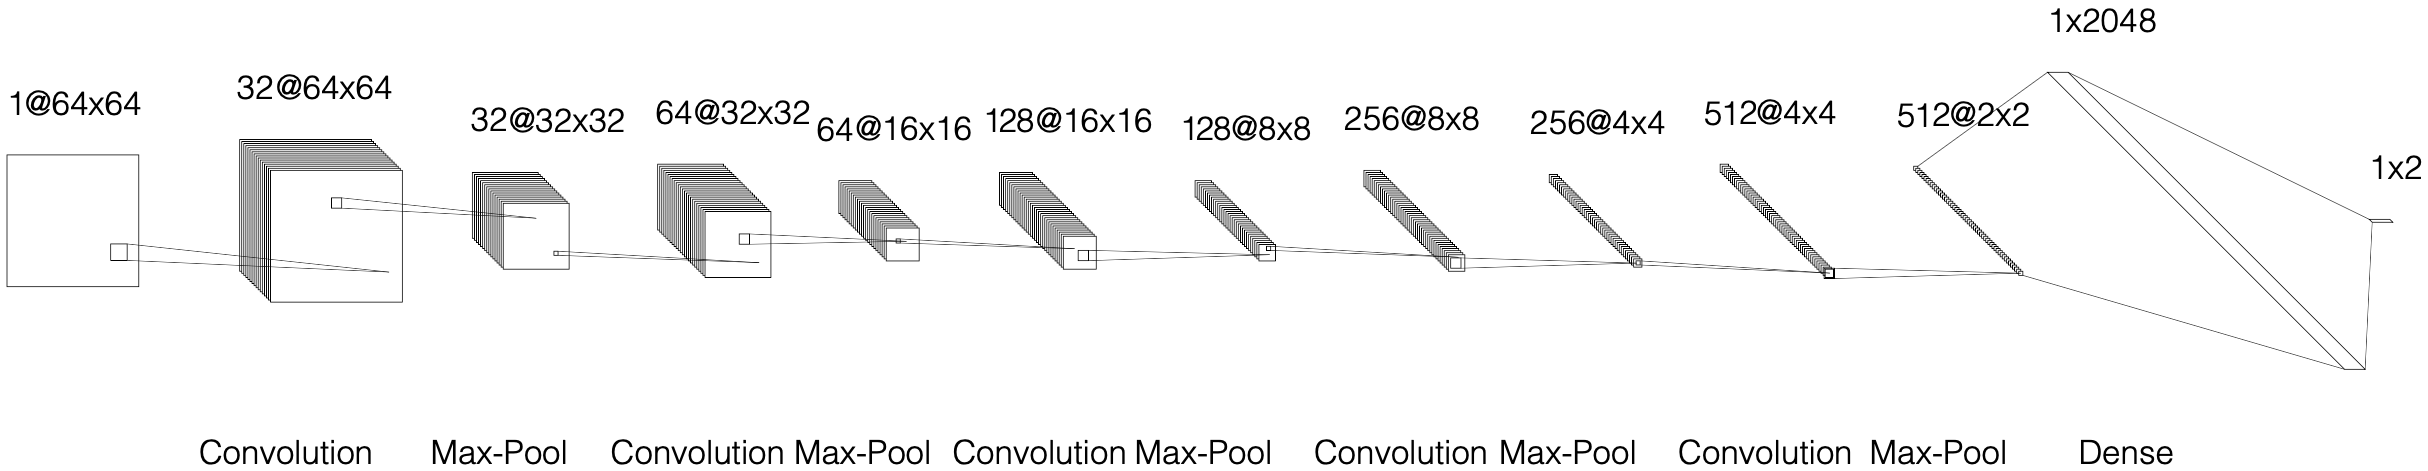
\includegraphics[scale=0.15]{pictures/CNN_our.png}}
	\caption{Architecture of the proposed CNN}
	\label{ris:CNN_our}
\end{figure}

\subsection{Performance metrics}
For the classification problem we use Accuracy.
Accuracy is defined by the formula:
\begin{equation}
Acc = \frac{\sum_{i=0}^{N} 1_{\{\hat{y}_i=y_i\}}}{N}
\end{equation}
where $N$ - number of samples, $\hat{y}$ - predicted label, $y$ - true label.

\subsection{Loss functions}
Weighted Binary Cross-Entropy both for segmentation and detection problems:
\begin{equation}
wBCE =-\frac{1}{N} \sum_{i=1}^{N} w_{1} \cdot y_{i} \cdot \log \left(p\left(\hat{y_{i}}\right)\right)
+ w_{2} \cdot \left(1-y_{i}\right) \cdot \log \left(1-p\left(\hat{y_{i}}\right)\right)
\end{equation}

\subsection{Existing CNNs}

We reimplemented CNN from \cite{Feng2017} with one difference: we used squared pictures (64x64 pixels) as an input, so we didn't implement Normalization layer (first layer in the Fig.~\ref{ris:CNN_feng2017}).
\begin{figure}[ht]
	\center{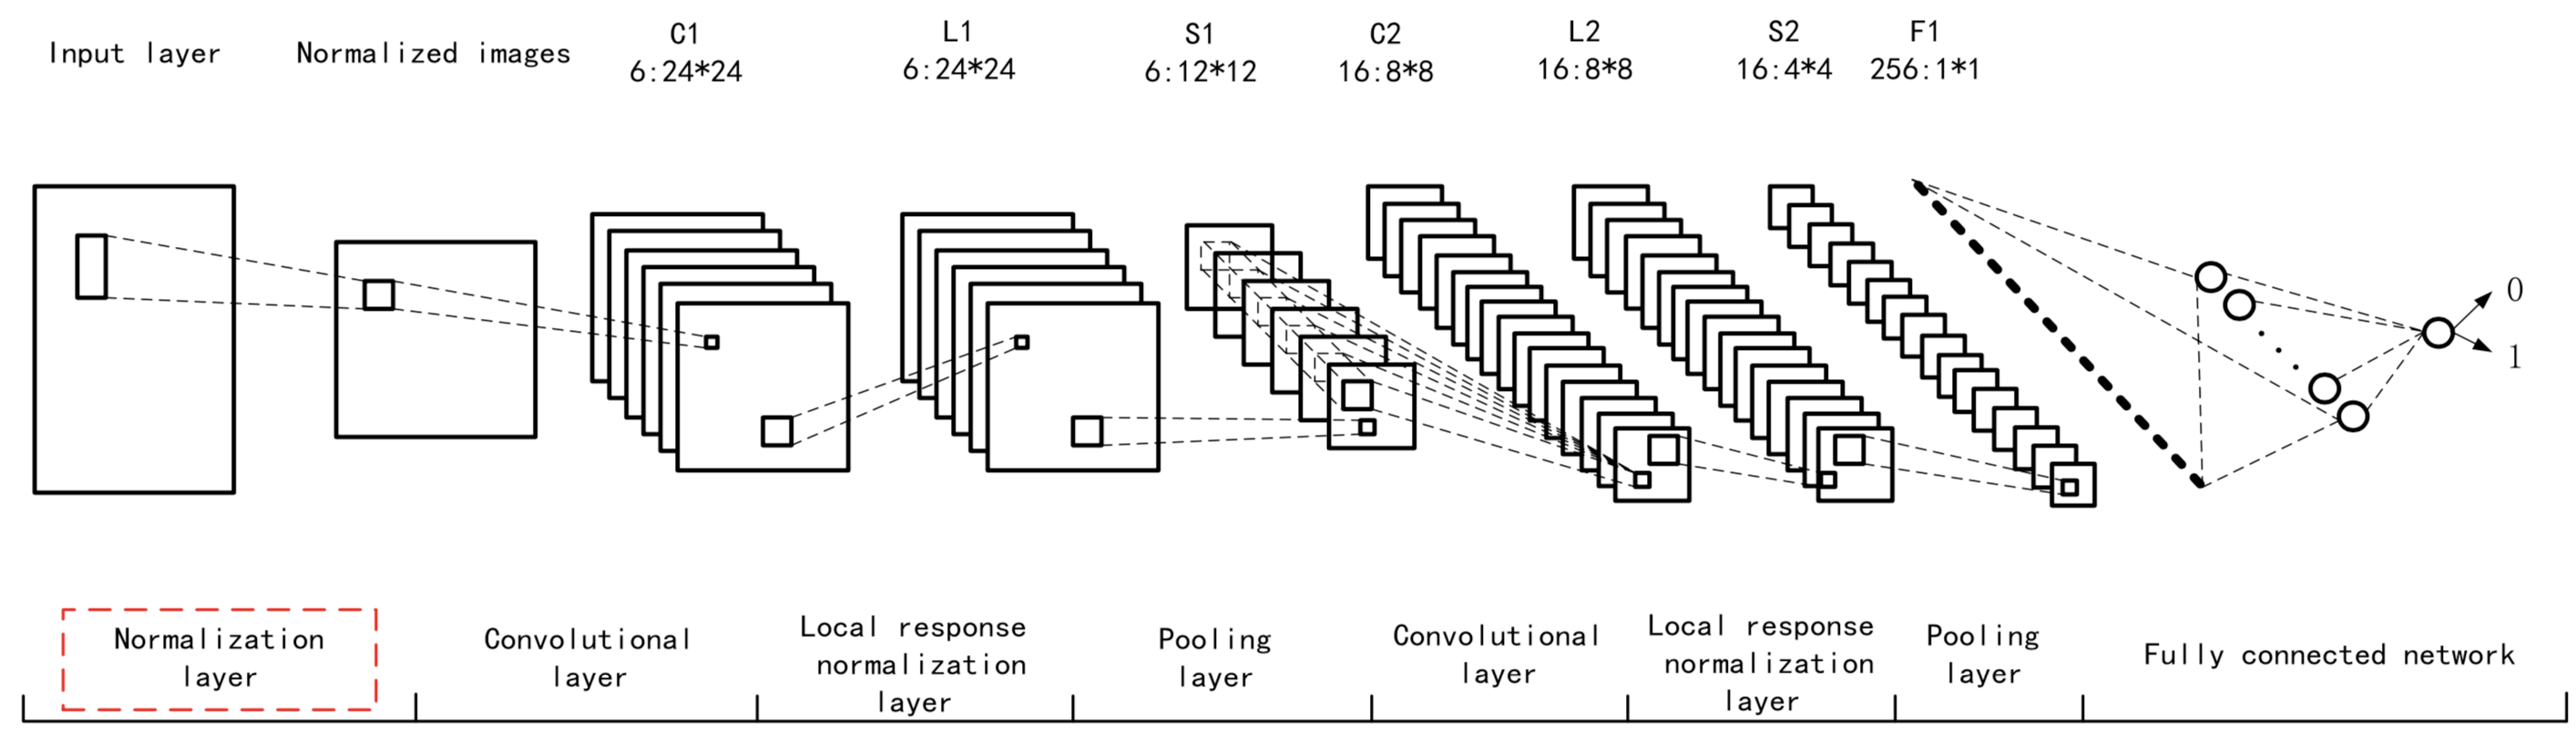
\includegraphics[scale=0.25]{pictures/CNN_feng2017.png}}
	\caption{Architecture of CNN from \cite{Feng2017}}
	\label{ris:CNN_feng2017}
\end{figure}
The interested reader can find all details and overall architecture parameters in \cite{Feng2017}.
From now on this CNN is marked as CNN-2 by the number of Convolutional layers.

We also reimplemented CNN from \cite{2020a}, which showed better results than pre-trained and fine-tuned OverFeatNet, VGGNet, GoogleNet networks.
The architecture is shown in Fig.~\ref{ris:raynet}.
Since our input size is smaller than in the original paper, we used smaller kernel size (3x3 instead of 7x7).
\begin{figure}[ht]
	\center{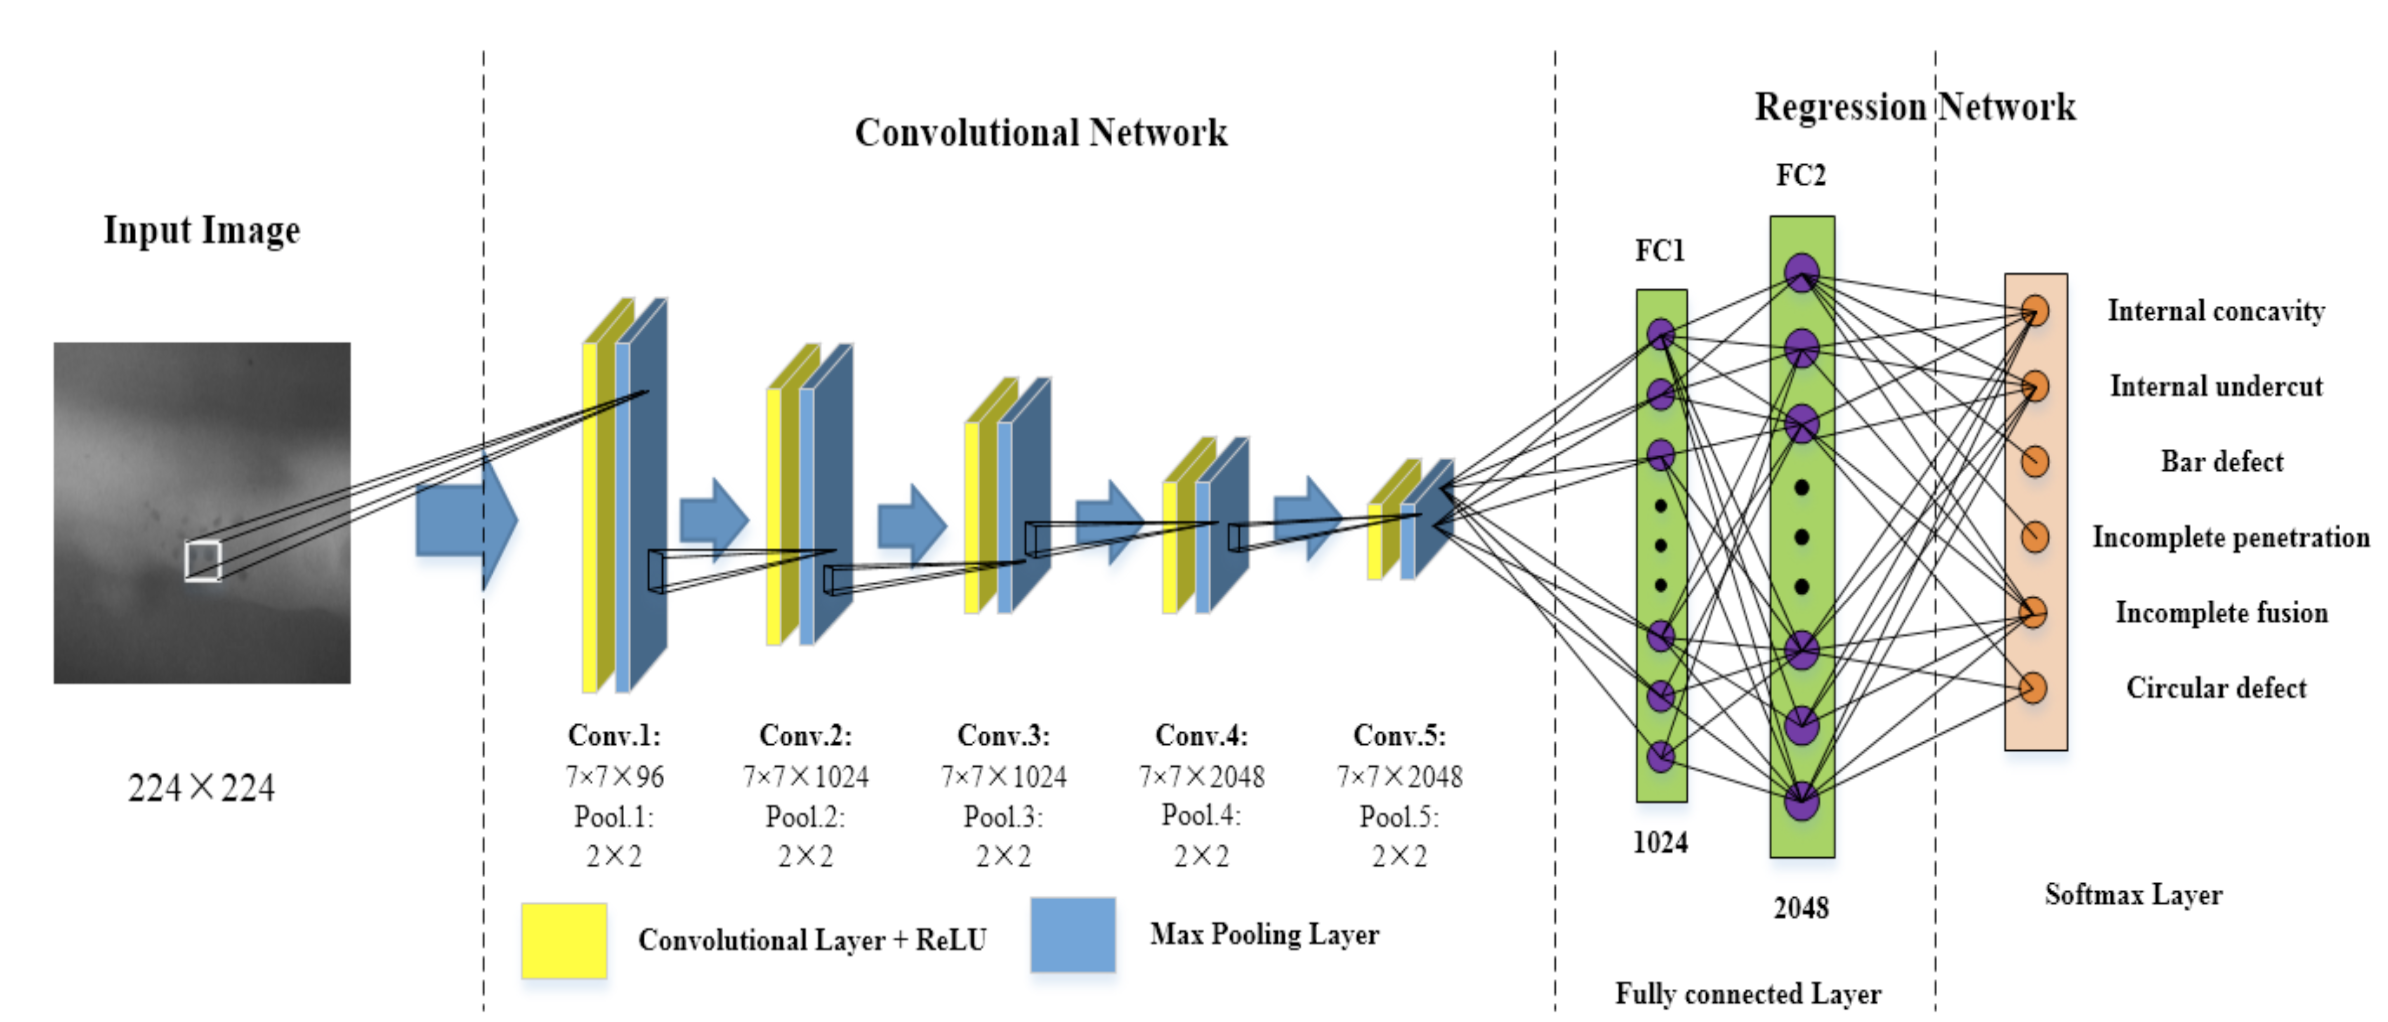
\includegraphics[scale=0.3]{pictures/raynet.png}}
	\caption{Architecture of CNN from \cite{2020a}}
	\label{ris:raynet}
\end{figure}
All details and CNN's parameters are presented in \cite{2020a}.
From now on this CNN is marked as RayNet.

